\documentclass[]{beamer}
\usetheme{presentation}
\usepackage[round]{natbib}
\usepackage{bibentry}
\definecolor{citecolor}{gray}{0.6}
\let\oldcitep\citep
\renewcommand{\citep}[1]{{\color{citecolor}\tiny\oldcitep{#1}}}
\nobibliography*
%\usepackage[cjk]{kotex}
%\usepackage{listings}
\usepackage{tikz}
\usetikzlibrary{arrows.meta}
\tikzset{
    invisible/.style={opacity=0},
    visible on/.style={alt={#1{}{invisible}}},
    alt/.code args={<#1>#2#3}{%
      \alt<#1>{\pgfkeysalso{#2}}{\pgfkeysalso{#3}} % \pgfkeysalso doesn't change the path
    },
}
% ----------------------------- Title & Author ------------------------------ %
\title{Causal Inference with Ordinal Outcomes}
\subtitle{Density Estimation Based Approach}
\author{Chanhyuk Park}
\institute{Washington University in St. Louis}
\date{}

\begin{document}
   \frame{\titlepage}
\begin{frame}{Motivation}
    \begin{itemize}
        \item Experiments to identify causal effects of treatments
        \pause 
        \item Outcomes are usually believed to be continuous in unidimensional space
            \begin{itemize}
                \item Approval ratings \citep{Canes-Wrone2002a, Kriner2009a}
                \item Policy preferences \citep{Scheve2001r, Mayda2005a, Wu2022a}
            \end{itemize}
    \end{itemize}

    \vspace{0.5cm}

    \centering
    % The Latent Axis Line and its label appear on Step 2 and persist.
    \only<2->{ 
        \begin{tikzpicture}[font=\sffamily, thick, scale=1.1]
            % --- Main Axis (Always Present in this block) ---
            \begin{scope} 
                \draw[very thick, black] (0,0) -- (10,0); 
                \foreach \x in {0, 10} \draw (\x, 0.1) -- (\x, -0.1);
                \node[above, yshift=5pt] at (5, 0.2) {\scriptsize\textbf{The True Outcome ($\boldsymbol{Y^{\ast}}$)}};
            \end{scope}
            \only<3>{
                \node at (1, -0.8) {\tiny\itshape Strongly Disagree}; \node at (3, -0.8) {\tiny\itshape Disagree}; \node at (5, -0.8) {\tiny\itshape Neither}; \node at (7, -0.8) {\tiny\itshape Agree}; \node at (9, -0.8) {\tiny\itshape Strongly Agree};
            }

            % --- Step 2: Index g_a (Naive/Positive ATE) ---
            \only<4>{
                \begin{scope}
                    \foreach \x [count=\i] in {2, 4, 6, 8}{ 
                        \draw (\x, 0.1) -- (\x, -0.1);
                        % \node[above] at (\x, 0.1) {\scriptsize $\alpha_{\i}$};
                    }
                    \draw (0,-0.2) to [out=-90, in=150] (1, -0.6); \draw (2,-0.2) to [out=-90, in=30] (1, -0.6); 
                    \draw (2,-0.2) to [out=-90, in=150] (3, -0.6); \draw (4,-0.2) to [out=-90, in=30] (3, -0.6); 
                    \draw (4,-0.2) to [out=-90, in=150] (5, -0.6); \draw (6,-0.2) to [out=-90, in=30] (5, -0.6); 
                    \draw (6,-0.2) to [out=-90, in=150] (7, -0.6); \draw (8,-0.2) to [out=-90, in=30] (7, -0.6); 
                    \draw (8,-0.2) to [out=-90, in=150] (9, -0.6); \draw (10,-0.2) to [out=-90, in=30] (9, -0.6); 
                    \node at (1, -0.8) {\tiny\itshape Strongly Disagree}; \node at (3, -0.8) {\tiny\itshape Disagree}; \node at (5, -0.8) {\tiny\itshape Neither}; \node at (7, -0.8) {\tiny\itshape Agree}; \node at (9, -0.8) {\tiny\itshape Strongly Agree};
                \end{scope}
            }

            % --- Step 3: Index g_b (Arbitrary/Flipped ATE) ---
            \only<5>{
                \begin{scope}
                    \draw[very thick] (0,0) -- (10,0); 
                    \foreach \x [count=\i] in {1.5, 4.5, 7.5, 9.5} {
                        \draw (\x, 0.1) -- (\x, -0.1);
                        % \node[above] at (\x, 0.1) {\scriptsize $\alpha_{\i}$};
                    }
                    \draw (0,-0.2) to [out=-90, in=150] (0.75, -0.6); \draw (1.5,-0.2) to [out=-90, in=30] (0.75, -0.6);
                    \draw (1.5,-0.2) to [out=-90, in=150] (3.0, -0.6); \draw (4.5,-0.2) to [out=-90, in=30] (3.0, -0.6);
                    \draw (4.5,-0.2) to [out=-90, in=150] (6.0, -0.6); \draw (7.5,-0.2) to [out=-90, in=30] (6.0, -0.6);
                    \draw (7.5,-0.2) to [out=-90, in=150] (8.5, -0.6); \draw (9.5,-0.2) to [out=-90, in=30] (8.5, -0.6);
                    \draw (9.5,-0.2) to [out=-90, in=150] (9.75, -0.6); \draw (10,-0.2) to [out=-90, in=30] (9.75, -0.6);
                    \node at (0.75, -0.8) {\tiny\itshape Strongly Disagree}; 
                    \node at (3.0, -0.8) {\tiny\itshape Disagree}; 
                    \node at (6.0, -0.8) {\tiny\itshape Neither}; 
                    \node at (8.5, -0.8) {\tiny\itshape Agree}; 
                    \node at (9.75, -0.8) {\tiny\itshape Strongly Agree};
                \end{scope}
            }
        \end{tikzpicture}
    }
\end{frame}

\begin{frame}{The Goal}
    \begin{itemize}
        \item<1-> \textit{\color<2->{purple}Identification} \\
            \only<2->{
                Naive causal identification with ordinal "index" fails \\
                \vspace{0.2cm}
                $\implies$ Alternative Estimand: \textcolor{purple}{Normalized Latent Treatment Effect}
            }
            \vspace{0.5cm}
        \item<1-> \textit{\color<3->{Orange}Estimation} \\
            \only<3->{
                Parametric ordered probit and logit with distributional assumptions \\
                \vspace{0.2cm}
                $\implies$ \textcolor{Orange}{Flexible, density estimation} based estimators
            }
    \end{itemize}
\end{frame}

\begin{frame}[label=main_cardinal]{Why Naive Identification Fails}
    \centering
    % --- Visualization Block (Appears from Click 2) ---
    \only<1->{ 
        \begin{tikzpicture}[font=\sffamily, thick, scale=1.1]
            % --- Main Axis (Always Present in this block) ---
            \begin{scope} 
                \draw[very thick, black] (0,0) -- (10,0); 
                \foreach \x in {0, 10} {
                    \draw (\x, 0.1) -- (\x, -0.1);
                }
                \node[above, yshift=5pt] at (5, 0.2) {\scriptsize\textbf{Policy Preference ($\boldsymbol{Y^{\ast}_{i} = \tau D_{i} + \varepsilon_i}$)}};
            \end{scope}

            % --- Step 2: Index g_a (Naive/Positive ATE) ---
            \only<5-7>{
                \begin{scope}[color=orange]
                    \foreach \x [count=\i, evaluate=\i as \idx using int(\i-1)] in {0, 2, 4, 6, 8, 10} {
                        \draw (\x, 0.1) -- (\x, -0.1);
                        \node[above] at (\x, 0.1) {\scriptsize $\alpha_{\idx}$};
                    }
                    \draw (0,-0.2) to [out=-90, in=150] (1, -0.6); \draw (2,-0.2) to [out=-90, in=30] (1, -0.6); 
                    \draw (2,-0.2) to [out=-90, in=150] (3, -0.6); \draw (4,-0.2) to [out=-90, in=30] (3, -0.6); 
                    \draw (4,-0.2) to [out=-90, in=150] (5, -0.6); \draw (6,-0.2) to [out=-90, in=30] (5, -0.6); 
                    \draw (6,-0.2) to [out=-90, in=150] (7, -0.6); \draw (8,-0.2) to [out=-90, in=30] (7, -0.6); 
                    \draw (8,-0.2) to [out=-90, in=150] (9, -0.6); \draw (10,-0.2) to [out=-90, in=30] (9, -0.6); 
                \end{scope}
                    \node at (1, -0.8) {\tiny\itshape Strongly Disagree}; \node at (3, -0.8) {\tiny\itshape Disagree}; \node at (5, -0.8) {\tiny\itshape Neither}; \node at (7, -0.8) {\tiny\itshape Agree}; \node at (9, -0.8) {\tiny\itshape Strongly Agree};
            }

            % --- Step 3: Index g_b (Arbitrary/Flipped ATE) ---
            \only<8-9>{
                \begin{scope}[color=Green]
                    \foreach \x [count=\i, evaluate=\i as \idx using int(\i-1)] in {0, 1.5, 4.5, 7.5, 9.5, 10} {
                        \draw (\x, 0.1) -- (\x, -0.1);
                        \node[above] at (\x, 0.1) {\scriptsize $\alpha_{\idx}$};
                    }
                    \draw (0,-0.2) to [out=-90, in=150] (0.75, -0.6); \draw (1.5,-0.2) to [out=-90, in=30] (0.75, -0.6);
                    \draw (1.5,-0.2) to [out=-90, in=150] (3.0, -0.6); \draw (4.5,-0.2) to [out=-90, in=30] (3.0, -0.6);
                    \draw (4.5,-0.2) to [out=-90, in=150] (6.0, -0.6); \draw (7.5,-0.2) to [out=-90, in=30] (6.0, -0.6);
                    \draw (7.5,-0.2) to [out=-90, in=150] (8.5, -0.6); \draw (9.5,-0.2) to [out=-90, in=30] (8.5, -0.6);
                    \draw (9.5,-0.2) to [out=-90, in=150] (9.75, -0.6); \draw (10,-0.2) to [out=-90, in=30] (9.75, -0.6);
                \end{scope}
                \node at (0.75, -0.8) {\tiny\itshape Strongly Disagree}; 
                \node at (3.0, -0.8) {\tiny\itshape Disagree}; 
                \node at (6.0, -0.8) {\tiny\itshape Neither}; 
                \node at (8.5, -0.8) {\tiny\itshape Agree}; 
                \node at (9.75, -0.8) {\tiny\itshape Strongly Agree};
            }
        \end{tikzpicture}
    }
    
    \vspace{0.2cm} % Space between visualization and table

    % --- TABLE 1: Click 1 (Only True Latent) ---
    \only<2-4>{
        \begin{tabular}{c|cc}
            \hline
            & $Y^{\ast}(0)$ & $Y^{\ast}(1)$ \\
            \hline
            A &\uncover<3->{0.8 & 1.2} \\
            B & \uncover<3->{0.4 & 0.6} \\
            C & \uncover<3->{1.9 & 2.2} \\
            D & \uncover<3->{1.5 & 1.7} \\
            E & \uncover<3->{2.5 & 2.4} \\
            \hline
        \end{tabular}
    }

    % --- TABLE 2: Click 2 (Latent + Index a) ---
    \only<5>{
        \begin{tabular}{c|cc|cc}
            \hline
            & $Y^{\ast}(0)$ & $Y^{\ast}(1)$ & \textcolor{orange}{$Y_{a}(0)$} & \textcolor{orange}{$Y_{a}(1)$} \\
            \hline
            A & 0.8 & 1.2 & Disagree & Neither \\
            B & 0.4 & 0.6 & Disagree & Disagree \\
            C & 1.9 & 2.2 & Neither & Agree \\
            D & 1.5 & 1.7 & Neither & Neither \\
            E & 2.5 & 2.4 & Agree & Agree \\
            \hline
        \end{tabular}
    }
    \only<6-7>{
        \begin{tabular}{c|cc|cc}
            \hline
            & $Y^{\ast}(0)$ & $Y^{\ast}(1)$ & \textcolor{orange}{$Y_{a}(0)$} & \textcolor{orange}{$Y_{a}(1)$} \\
            \hline
            A & 0.8 & 1.2 & 2 & 3 \\
            B & 0.4 & 0.6 & 2 & 2 \\
            C & 1.9 & 2.2 & 3 & 4 \\
            D & 1.5 & 1.7 & 3 & 3 \\
            E & 2.5 & 2.4 & 4 & 4 \\
            \hline
        \end{tabular}
    }

    % --- TABLE 3: Click 3 (Latent + Index b) ---
    \only<8>{
        \begin{tabular}{c|cc|cc}
            \hline
            & $Y^{\ast}(0)$ & $Y^{\ast}(1)$ & \textcolor{Green}{$Y_{b}(0)$} & \textcolor{Green}{$Y_{b}(1)$} \\
            \hline
            A & 0.8 & 1.2 & Disagree & Disagree \\
            B & 0.4 & 0.6 & Disagree & Disagree \\
            C & 1.9 & 2.2 & Neither & Neither \\
            D & 1.5 & 1.7 & Neither & Neither \\
            E & 2.5 & 2.4 & Agree & Neither \\
            \hline
        \end{tabular}
    }
    \only<9>{
        \begin{tabular}{c|cc|cc}
            \hline
            & $Y^{\ast}(0)$ & $Y^{\ast}(1)$ & \textcolor{Green}{$Y_{b}(0)$} & \textcolor{Green}{$Y_{b}(1)$} \\
            \hline
            A & 0.8 & 1.2 & 2 & 2 \\
            B & 0.4 & 0.6 & 2 & 2 \\
            C & 1.9 & 2.2 & 3 & 3 \\
            D & 1.5 & 1.7 & 3 & 3 \\
            E & 2.5 & 2.4 & 4 & 3 \\
            \hline
        \end{tabular}
    }

    \vspace{0.2cm}
    \only<4-9>{
        \begin{itemize}
            \item $\tau = \E{Y^{\ast}(1)} - \E{Y^{\ast}(0)} \approx \textbf{+0.2}$ 
                \only<7>{
                \item $\tau_{a} = \E{\textcolor{orange}{Y_{a}(1)}} - \E{\textcolor{orange}{Y_{a}(0)}} \approx \textcolor{orange}{\textbf{+0.4}}$
                }
                \only<9>{
                \item $\tau_{b} = \E{\textcolor{Green}{Y_{b}(1)}} - \E{\textcolor{Green}{Y_{b}(0)}} \approx \textcolor{Green}{\textbf{-0.2}}$
                }
        \end{itemize}
    }
    \only<9>{
    \hfill\hyperlink{appx_binary}{\beamergotobutton{Binarization}}
    }
\end{frame}

\begin{frame}[label=main_id]{Identification Through Link Function}
    \begin{itemize}[<+->]
        \item Cumulative probabilities \textcolor{orange}{$\P{Y \le j}$} (e.g. $\P{Y \le \text{Agree}}$
        \item If we can \textit{map} these probabilities to the $Y^{\ast}$ space
        \item \textcolor{Green}{Link Function = CDF of $\varepsilon_i$ ($F_{\varepsilon_{i}}$)} does this:
            $$
                F_{\varepsilon_{i}}^{-1}\bigl(\textcolor{orange}{\P{Y_{i} \le j}}\bigl) = \underbrace{\alpha_{j} - \tau D_{i}}_{\text{Defined in $Y^*$ space}}
            $$
        \item \textcolor{purple}{Key Assumption}: Distribution of $\varepsilon_i$ is \textit{known}
            $$ 
                \underbrace{F_{\varepsilon_{i}}^{-1}(\P{Y_{i}(0) \le j})}_{\text{Control}} - \underbrace{F_{\varepsilon_{i}}^{-1}(\P{Y_{i}(1) \le j})}_{\text{Treated}} = \tau 
            $$
    \end{itemize}
    \only<5>{
        \hfill\hyperlink{appx_id}{\beamergotobutton{Little More on Link Function}}
    }
\end{frame}

\begin{frame}{New Estimands: Normalized Treatment Effect}
    \begin{itemize}[<+->]
        \item One caveat: for a positive constant $C$,
            $$
            \begin{aligned}
                \P{Y_{i} \le j}
                % &= \P{Y^{\ast}_{i} \le \alpha_{j}} \\
                % &= \P{C\cdot Y^{\ast}_{i} \le C \cdot \alpha_{j}} \\
                &= \P{\tau D_{i} + \varepsilon_i \le \alpha_{j}} \\
                &= \P{C\cdot \tau D_{i} + C \cdot \varepsilon_i \le C \cdot \alpha_{j}} \\
            \end{aligned}
            $$ 
        \item $\tau$ becomes indistinguishable from $C \cdot \tau$
        \item Normalization to cancel out $C$
        \begin{enumerate}
            \item {\color<6->{blue} Scale to fix $\sigma_{\varepsilon_{i}} = 1$} \\
                \only<6->{\color{blue}
                    \vspace{0.2cm}
                    $\implies \frac{C \cdot \tau}{C \cdot \sigma_{ \varepsilon_{i}}} = \frac{\tau}{\sigma_{\varepsilon_{i}}}$ is identified
                    \vspace{0.2cm}
                }
            \item<4-5> If there are multiple treatments, fixing $\tau_{a} = 1$
        \end{enumerate}   
    \end{itemize}
\end{frame}

\begin{frame}{How Can We Estimate?}
    \begin{itemize}[<+->]
        \item The key is \textcolor{Green}{Distribution of $\varepsilon_{i}$}
        \item Ordered Probit, Ordered Logit, and IRT \\
        \item They assume a specific the CDF $F_{\varepsilon_i}$ $\rightarrow$ MLE
        \item Distributional Assumption can be violated
            \begin{itemize}
                \item Pure misspecification
                \item Unaccounted covariates
                \item[] $\implies$ Become \textit{\textcolor{red}{inconsistent}} 
            \end{itemize}
            \vspace{0.3cm}
        \item \textcolor{blue}{Two Flexible Estimators} without rigid Distributional Assumptions
    \end{itemize}
\end{frame}

\begin{frame}[label=main_density]{Alternative: Estimate the Distribution}
    \begin{itemize}
        \item<1-> Estimated $\hat{F}_{\varepsilon_{i}}$ from the Data
        \item<2-> Nonparametric method: \textcolor{purple}{Kernel Density Estimation}
            \begin{itemize}
                \item Use Kernels to smooth each observations
            \end{itemize}
            \vspace{0.5cm}
            
        \item<3-> Parametric Generative Model: \textcolor{Orange}{Normalizing Flows} 
            \begin{itemize}
                \item Transform complex distributions to simple one
            \end{itemize}
            \vspace{0.5cm}
        \item<4-> Same MLE
    \end{itemize}
    \only<4>{
        \hfill\hyperlink{appx_density}{\beamergotobutton{Little More on Density Estimation}}
    }
\end{frame}

\begin{frame}{Simulation Setting}
    \begin{figure}
        \only<2>{
            \includegraphics[width=0.95\textwidth]{../figures/latent_zoom_lognormal_N1000000.pdf}
        }
        \only<3>{
            \includegraphics[width=0.95\textwidth]{../figures/latent_space_lognormal_N1000000.pdf}
        }
    \end{figure}
\end{frame}

\begin{frame}{Simulation Results: Bias and Simulation SD}
    \centering
    
    % --- Plot Area ---
    \begin{figure}
        % Click 1: OLS only
        \only<2>{
            \includegraphics[width=0.9\textwidth]{../figures/bias_lognormal1.pdf}
        }
        % Click 2: OLS + Parametric
        \only<3>{
            \includegraphics[width=0.9\textwidth]{../figures/bias_lognormal2.pdf}
        }
        % Click 3: OLS + Parametric + Density
        \only<4>{
            \includegraphics[width=0.9\textwidth]{../figures/bias_lognormal3.pdf}
        }
    \end{figure}
\end{frame}

\begin{frame}{Replication -- \citet{Mattingly2025a}}
    \begin{itemize}[<+->]
        \item State-produced promotional media $\rightarrow$ preference on political system
        \item 19 different countries with $n = 6,000$
        \item Three treatments:
            \begin{enumerate}
                \item China: Two CCP produced videos
                \item USA: Two US produced videos
                \item Competition: One from CCP and the other from US
            \end{enumerate}
        \item Outcome: Preference on Political System \\
            \hspace{1.25cm}\textit{Strongly Prefer the US} to \textit{Strongly Prefer China}
    \end{itemize}
\end{frame}

\begin{frame}{Replication Results}
    \begin{table}[!htb]\scriptsize
        \begin{center}
            % Use a fixed 6-column spec: l c c c c c
            \begin{tabular}{l c | c c c c }
                \\ [-1.8ex] \hline\\ [-1.8ex]
                & ATE & \multicolumn{4}{c}{\uncover<2->{NLTE}} \\
                \\ [-1.8ex]\cline{2-6} \\ [-1.8ex]
                & Original -- OLS & \uncover<2->{Ordered Logit} & \uncover<2->{Ordered Probit} & \uncover<3->{KDE-based} & \uncover<3->{NF-based} \\
                \\ [-1.8ex] \hline\\ [-1.8ex]

                % China Row
                China & $1.04^{\ast\ast\ast}$ & \uncover<2->{$0.73^{\ast\ast\ast}$} & \uncover<2->{$0.76^{\ast\ast\ast}$} & \uncover<3->{$0.36^{\ast\ast\ast}$} & \uncover<3->{$0.37^{\ast\ast\ast}$} \\
                & $(0.05)$ & \uncover<2->{$(0.04)$} & \uncover<2->{$(0.04)$} & \uncover<3->{$(0.07)$} & \uncover<3->{$(0.04)$} \\

                % USA Row
                USA & $-0.43^{\ast\ast\ast}$ & \uncover<2->{$-0.35^{\ast\ast\ast}$} & \uncover<2->{$-0.38^{\ast\ast\ast}$} & \uncover<3->{$-0.18^{\ast\ast\ast}$} & \uncover<3->{$-0.17^{\ast\ast\ast}$} \\
                & $(0.04)$ & \uncover<2->{$(0.04)$} & \uncover<2->{$(0.04)$} & \uncover<3->{$(0.05)$} & \uncover<3->{$(0.03)$} \\

                % Competition Row
                Competition & $0.36^{\ast\ast\ast}$ & \uncover<2->{$0.21^{\ast\ast\ast}$} & \uncover<2->{$0.25^{\ast\ast\ast}$} & \uncover<3->{$0.13^{\ast}$} & \uncover<3->{$0.11^{\ast\ast}$} \\
                & $(0.05)$ & \uncover<2->{$(0.04)$} & \uncover<2->{$(0.04)$} & \uncover<3->{$(0.06)$} & \uncover<3->{$(0.04)$} \\

                \\ [-1.8ex] \hline\\ [-1.8ex]
                \multicolumn{6}{l}{\hfill\scriptsize{$^{***}p<0.001$; $^{**}p<0.01$; $^{*}p<0.05$}}
            \end{tabular}
        \end{center}
    \end{table}
\end{frame}

\begin{frame}{Conclusion}
    \begin{itemize}
        \item<1-> \textit{\color<2->{purple}Identification} \\
            \only<2->{
                Naive use of ordinal "index" can not give us what we want \\
                \vspace{0.2cm}
                $\implies$ Alternative Estimand: \textcolor{purple}{Normalized Latent Treatment Effect}
            }
            \vspace{0.5cm}
        \item<1-> \textit{\color<3->{Orange}Estimation} \\
            \only<3->{
                Parametric ordinal regressions require strong assumptions \\
                \vspace{0.2cm}
                $\implies$ \textcolor{Orange}{KDE} or \textcolor{Orange}{Normalizing Flows} based estimators
            }
    \end{itemize}
\end{frame}

\appendix

\begin{frame}[label=appx_id]{More on Link Function}
    \begin{tikzpicture}[font=\sffamily, thick, scale=1.1]
        \only<2-6>{
            \centering
            \begin{scope}
                \draw[very thick] (0,0) -- (10,0); 

                \node[above, yshift=5pt] at (5, 0.2) {\scriptsize\textbf{The True Outcome ($\boldsymbol{Y^{\ast}_{i} = \tau D_{i} + \varepsilon_i}$)}};
                \only<3-6>{
                    \node[above, yshift=5pt] at (5, 0.2) {\scriptsize\textbf{The True Outcome (\textcolor{orange}{$\boldsymbol{Y^{\ast}_{i} = \tau D_{i} + \varepsilon_i}$})}};
                }
                \foreach \x [count=\i, evaluate=\i as \idx using int(\i-1)] in {0, 2, 4, 6, 8, 10} {
                    \draw (\x, 0.1) -- (\x, -0.1);
                    \node[above] at (\x, 0.1) {\scriptsize $\alpha_{\idx}$};
                } 
                \only<2-6>{
                    \node[above] at (8, 0.1) {\scriptsize \textcolor{red}{$\alpha_{4}$}};
                }
                % Brackets and Category Labels
                \draw (0,-0.2) to [out=-90, in=150] (1, -0.6); \draw (2,-0.2) to [out=-90, in=30] (1, -0.6); 
                \draw (2,-0.2) to [out=-90, in=150] (3, -0.6); \draw (4,-0.2) to [out=-90, in=30] (3, -0.6); 
                \draw (4,-0.2) to [out=-90, in=150] (5, -0.6); \draw (6,-0.2) to [out=-90, in=30] (5, -0.6); 
                \draw (6,-0.2) to [out=-90, in=150] (7, -0.6); \draw (8,-0.2) to [out=-90, in=30] (7, -0.6); 
                \draw (8,-0.2) to [out=-90, in=150] (9, -0.6); \draw (10,-0.2) to [out=-90, in=30] (9, -0.6); 

                \node at (1, -0.8) {\tiny\itshape Strongly Disagree}; 
                \node at (3, -0.8) {\tiny\itshape Disagree}; 
                \node at (5, -0.8) {\tiny\itshape Neither}; 
                \node at (7, -0.8) {\tiny\itshape Agree}; 
                \node at (9, -0.8) {\tiny\itshape Strongly Agree};
            \end{scope}
        }
    \end{tikzpicture}
    \begin{itemize}[<+->]
        \only<1, 7->{
            \item Cumulative probabilities such as $\P{Y \le \text{Agree}}$
        }
        \item \textcolor{Green}{Link function = CDF of the error term( $F_{\varepsilon_{i}}$ )}
            $$
            \begin{aligned}
                \only<2-7>{
                F_{\varepsilon_{i}}^{-1}\left(\P{Y_{i} \le \text{Agree}}\right) 
                \only<2-6>{
                &=  
                    F_{\varepsilon_{i}}^{-1}\left(\P{Y^{\ast}_{i} \le \textcolor{red}{\alpha_{4}}}\right) \\
                }
                    \only<3-6>{
                    &=  
                    F_{\varepsilon_{i}}^{-1}\left(\P{\textcolor{orange}{\tau D_{i} + \varepsilon_i} \le \alpha_{4}}\right) \\
                }
                    \only<4-6>{
                        &=  
                        F_{\varepsilon_{i}}^{-1}\left(\P{\varepsilon_i \le \alpha_{4} - \tau D_{i}}\right) \\
                    }
                    \only<5-6>{
                        &=  
                        F_{\varepsilon_{i}}^{-1}\left(F_{\varepsilon_i} \left(\alpha_{4} - \tau D_{i}\right)\right) \\
                    }
                    \only<6-7>{
                        &= \alpha_{4} - \tau D_i
                    }
                }
            \end{aligned}
            $$ 
        \only<1, 7->{
            \item<7-> Suppose we know $F_{\varepsilon_i}$:
                $$ \underbrace{F_{\varepsilon_{i}}^{-1}(\P{Y_{i}(0) \le \text{Agree}})}_{\text{Control}} - \underbrace{F_{\varepsilon_{i}}^{-1}(\P{Y_{i}(1) \le \text{Agree}})}_{\text{Treated}} = \tau $$
        }
    \end{itemize}
    \hyperlink{main_id}{\beamerreturnbutton{Back}}
\end{frame}


\begin{frame}[label=appx_density]{Little More on Density Estimation}
    \begin{itemize}
        \item \textcolor{purple}{Kernel Density Estimation} \\
        Let $V_i(\beta,\tau) = f(X_i,\beta) + D_i^\top\tau$ \\
        By the Bayes' rule,
        $$
            \mathbb{P}(Y_i \le j \mid V_i = v)
                = \frac{ \P{Y_{i} \le j}  g_1(v \mid Y \le j) }{
                    \P{Y_{i} \le j}  g_1(v \mid Y \le j)
                    + \P{Y_{i} > j}  g_0(v \mid Y > j)
                }
        $$ \\
        Estimate $g_{i}$ using KDE

        $$
            \hat{g}_{1}(v \mid Y \le j)
            = \frac{1}{n_1(j) h_{1j}} \sum_{i: Y_i \le j}
            K\left( \frac{v - V_i}{h_{1j}} \right)
        $$
        $$
            \hat{g}_{0}(v \mid Y > j)
            = \frac{1}{n_0(j) h_{0j}} \sum_{i: Y_i > j}
            K\left( \frac{v - V_i}{h_{0j}} \right)
            $$
    \end{itemize}
    \hyperlink{main_density}{\beamerreturnbutton{Back}}
\end{frame}
            
\begin{frame}{Little More on Density Estimation}
    \begin{itemize}
        \item \textcolor{Orange}{Normalizing Flows} 
                \begin{itemize}
                    \item Use the change-of-variable formula
                        $$
                        f_\theta(\varepsilon)
                        = f_Z\bigl(T_\theta^{-1}(\varepsilon)\bigr)
                        \left|\det \left( \frac{\partial T_\theta^{-1}(\varepsilon)}{\partial \varepsilon} \right) \right|,
                        $$
                    \item $\varepsilon_i = T_\theta(Z_i)$
                    \item $T_{\theta}$ is a set of \textit{invertible} transformation
                    \item Maps $\varepsilon_i$ to simple $Z$ (e.g. Standard Normal)
                    \item Estimate based on $Z$ and then translate it back to $\varepsilon_i$
                \end{itemize}
    \end{itemize}
    \hyperlink{main_density}{\beamerreturnbutton{Back}}
\end{frame}

\begin{frame}[label=appx_binary]{Why Not Just Use Binary Outcomes?}
    \begin{itemize}
        \item Loss of Power
            \begin{itemize}
                \item Collapsing categories wastes information
                \item Require larger samples ($\approx 5\times$)
            \end{itemize}
        \vspace{0.4cm}
        \item Aggregation Bias
            \begin{itemize}
                \item Arbitrary grouping may fail to identify effects or \textit{flip the sign} of the effect
                \item Depends on shifts in middle categories
            \end{itemize}
        \vspace{0.4cm}
        \item Example:
            \begin{itemize}
                \item Treatment moves "Strongly Disagree" $\rightarrow$ "Disagree"
                \item Binary ("Positive" vs "Negative") sees \textit{zero} effect
                \item Ordinal model captures the improvement
            \end{itemize}
    \end{itemize}
    \hyperlink{main_cardinal}{\beamerreturnbutton{Back}}
\end{frame}

\bibliographystyle{plainnat}
\nobibliography{/Users/chanhyuk/Documents/MyLibrary}

\end{document}
